\section{Numerical Results}
\label{sec:results} %2.5 pages

\subsection{Experimental Setup}

All experiments were conducted on a 12-node cluster at the Center for High Performance Computing (CHPC) at 
the University of Utah. Each node consists of a dual-socket Intel Xeon Haswell processors with 14 cores each 
for a total of 28 cores and 128GB per node. 

%The lazy-updates experiments have been done on Chiron servers in \textit{SCI - University of Utah}.
%They are performed using a 64 cores Intel Xeon x7560 2.27GHz (128 with HT) machine with 504GB of RAM and with OS openSUSE 42.1.
% The weak and strong scaling experiments are measured on Kingspeak servers located in \textit{CHPC - University of Utah}. Each node has two sockets, with 14 cores on each socket.

Two sets of experiments have been done for this section. The first experiment shows how lazy-update for AMG behaves on a matrix
generated from a 2D mesh in \textit{Nektar++} which is shown in Figure \ref{fig:mesh}. The mesh has order 7 and has triangles and
quads and is a challenging mesh for AMG. The generated matrix is of size 870 by 870 and has 33761 nonzeros.

The AMG hierarchy is created on an initial matrix $A$. Then the linear system 
$Ax = b$ is solved and number of vcycle iterations that it takes for the solve phase is written on the plot.
Then, the difusion coefficients change based on a sine function to generate another matrix ($B_1$) which is slightly 
different from the initial one. The number of iterations to solve the system $B_1x = b$ is shown on the plot.
The same process is repeated for multiple matrices.

The second set of experiments shows weak scaling and strong scaling of AMG as a preconditioner on 2D Poisson problem.
One MPI task is assigned to each socket, so each node has two MPI tasks, corresponding to our hardware confguration. 
%(except the first one, which has one MPI task in total).
The number of OpenMP threads on each socket is 14.
For the weak scaling each processor has almost 262k degree of freedom. In the strong scaling the total degree of freedom for all
the experiments is $1048000$.

\begin{figure}[H]
 \centering
 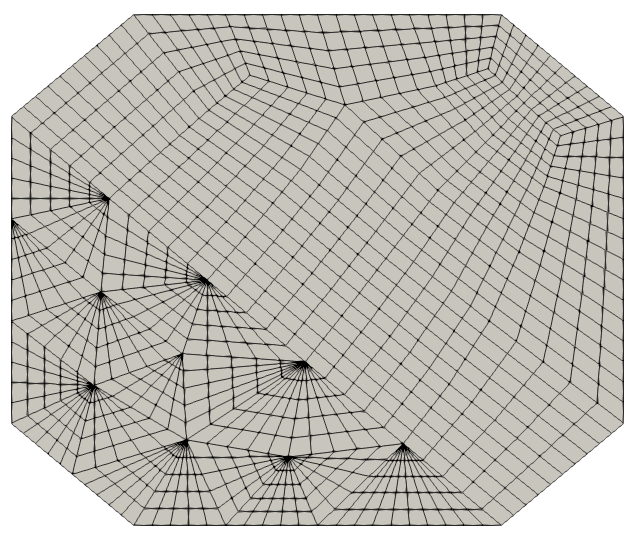
\includegraphics[width=8cm,height=7cm]{./figures/mesh.png}
 \caption{The mesh that is used for the sinusoidal diffusion coefficient change experiment.}
 \label{fig:mesh}
\end{figure}

\subsection{Results}

Figure~\ref{fig:strategy1} shows the lazy-update AMG using the first strategy.
The blue and red lines show how the coefficients are generated based on a sine function to create new matrices $B_i$.
By using strategy1, only $As[1]$ of the whole AMG hierarchy will be updated to solve each new linear system $B_ix = b$.
The plot shows that by saving the time using the same AMG hierarchy from the initial matrix, only a couple more (at most 6)
iterations is required to solve a linear system similar to the initial one. So, even though we need to spend a little more
time in the solve phase, almost the entire setup phase can be avoided.

Figure~\ref{fig:strategy2} shows a similar result for the second strategy. Here, all $As$ are updated in the setup phase
for the new matrices, so more setup time comparing to the first strategy is required, but at most 4 additional iterations are required during the solve phase.

\begin{figure}[H]
 \centering
 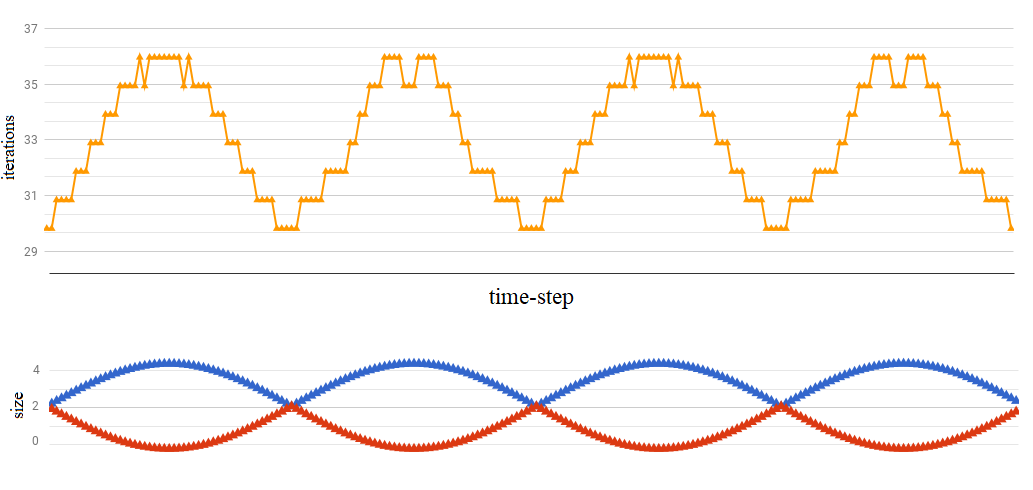
\includegraphics[width=10cm,height=5cm]{./figures/update2-3.png}
 \caption{Strategy1: The entire AMG hierarchy is re-used without incurring the cost of additional setup, except for the fine matrix. $As[1]$ is the only part that gets updated.
          The orange marks show how many iterations is required to achieve $10^{-12}$ relative tolerance.
          Each orange triangle corresponds to the number of iterations required to solve the system for a new updated matrix.
          The blue (red) triangles are the maximum (minimum) diffusion coefficients used to generate the new matrices.}
 \label{fig:strategy1}
\end{figure}

\begin{figure}[H]
 \centering
 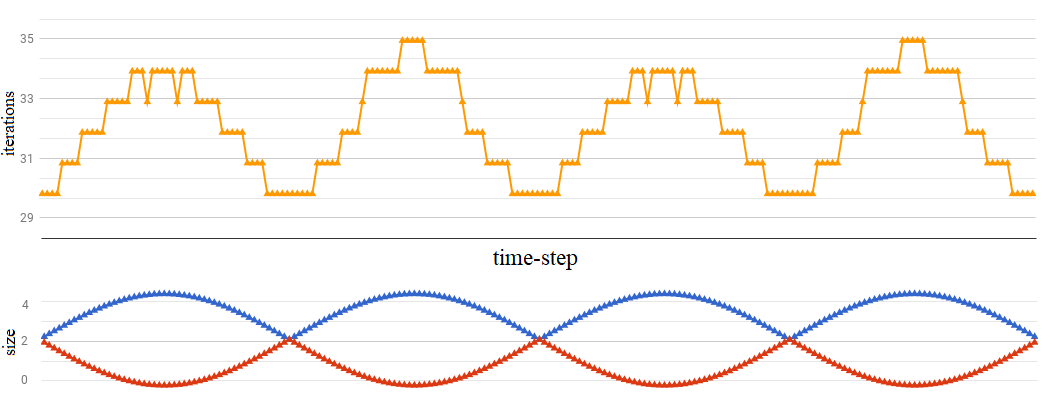
\includegraphics[width=10cm,height=5cm]{./figures/update3-3.png}
 \caption{Strategy2: The aggregations is not updated, but the coarse grid matrices are recomputed. 
 All $As$ matrices get updated, but $Ps$ and $Rs$ are used from the initial AMG hierarchy.
          The orange marks show how many iterations is required to achieve $10^{-12}$ relative tolerance.
          Each orange triangle corresponds to the number of iterations required to solve the system for a new updated matrix.
          The blue (red) triangles are the maximum (minimum) diffusion coefficients used to generate the new matrices.}
 \label{fig:strategy2}
\end{figure}

Figure \ref{fig:solvesetup} shows the weak and strong scalability of the solve and setup phases,
for the 2D Poisson problem. One can easily notice that the setup time takes more than 17 times more time than the setup phase for this experiment.
From that, it is obvious why we accept a small increase in the solve time, to avoid doing some steps of the setup phase in the strategies we discussed.

\begin{figure}[H]
 \centering
 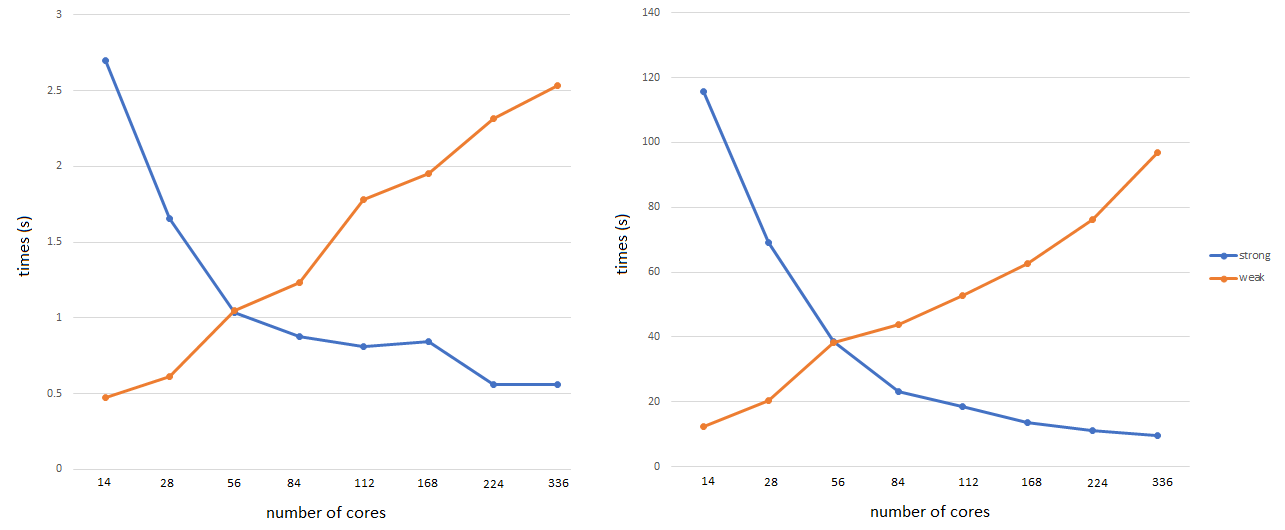
\includegraphics[width=13cm,height=5cm]{./figures/solvesetup.png}
 \caption{strong (blue) and weak scaling (orange) of the AMG solve (left) and setup (right) phases.
          The setup phase takes significantly more time than the solve step.}
 \label{fig:solvesetup}
\end{figure}
